\documentclass[11pt, letterpaper]{article}
% --- UNIVERSAL PREAMBLE BLOCK ---
\usepackage[a4paper, top=2cm, bottom=2cm, left=1.5cm, right=1.5cm]{geometry}
\usepackage{amsmath}
\usepackage{tikz}
\usetikzlibrary{shapes.geometric}
\usepackage{tcolorbox}
\usepackage{enumitem}
\setlist[itemize]{label=-}

% --- TIKZ NODE STYLES ---
\tikzset{
  maxnode/.style={regular polygon, regular polygon sides=3, draw, minimum size=1cm, inner sep=0pt, fill=blue!20, font=\bfseries\small, align=center},
  minnode/.style={regular polygon, regular polygon sides=3, shape border rotate=180, draw, minimum size=1cm, inner sep=0pt, fill=red!20, font=\bfseries\small, align=center},
  chancenode/.style={circle, draw, minimum size=0.8cm, inner sep=0pt, fill=green!20, font=\bfseries\small, align=center},
  terminal/.style={rectangle, draw, minimum size=0.6cm, inner sep=3pt, fill=purple!20, font=\bfseries\small, align=center},
  prob/.style={font=\scriptsize\bfseries, text=black!70}
}

\title{\textbf{CS 471 -- Lesson 8 In-Class Worksheet}}
\author{Adversarial and Stochastic Decision Making}
\date{}

\begin{document}

\maketitle

% ---------------------------------------------------------
% SECTION 1: WORKSHEET
% ---------------------------------------------------------
\section*{Guided In-Class Worksheet (Instructor-Led)}

\textbf{Objective:} Explain minimax decision-making and zero-sum interactions in competitive environments, and describe expectimax and decision-making within stochastic environments.

\vspace{0.5em}
\noindent\textbf{Symbology Legend}:
\begin{itemize}
    \item \textbf{Upward Triangle:} Max Agent Decision (You)
    \item \textbf{Downward Triangle:} Min Agent Decision (Adversary)
    \item \textbf{Circle:} Chance Node (Uncertain Outcomes)
    \item \textbf{Square:} Terminal Utility / State Value
\end{itemize}

\subsection*{Part 1: Adversarial Search (Minimax)}

\noindent\textbf{Scenario 1:} As a cadet at the Air Force Academy, you are competing in a simulated zero-sum wargame. You are commanding a blue-force drone swarm (Max) attempting to maximize the number of enemy targets destroyed. An intelligent red-force commander (Min) is actively deploying countermeasures to minimize your success. This is a deterministic, zero-sum game. 

\vspace{0.5em}
\noindent\textbf{Directions:} Minimax values are computed recursively, working backwards from the terminal states. Trace the 5-layer minimax tree below to find the optimal policy against a rational adversary.

\begin{center}
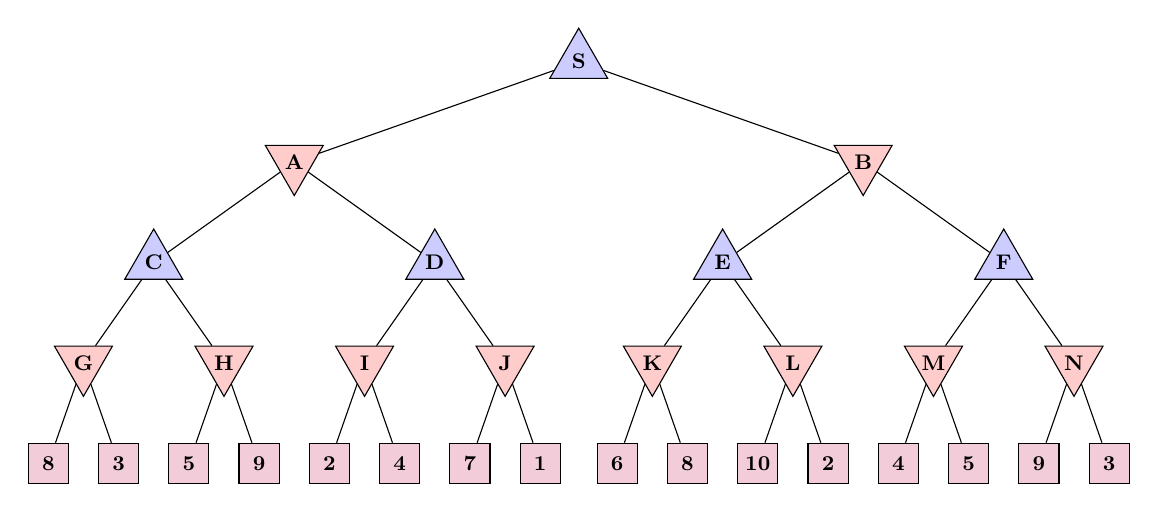
\begin{tikzpicture}[level distance=1.5cm,
  level 1/.style={sibling distance=8.5cm},
  level 2/.style={sibling distance=4.2cm},
  level 3/.style={sibling distance=2.1cm},
  level 4/.style={sibling distance=1.05cm},
  scale=0.85, every node/.style={transform shape}]
  
  \node[maxnode] {S}
    child {node[minnode] {A}
      child {node[maxnode] {C}
        child {node[minnode] {G}
          child {node[terminal] {8}}
          child {node[terminal] {3}}
        }
        child {node[minnode] {H}
          child {node[terminal] {5}}
          child {node[terminal] {9}}
        }
      }
      child {node[maxnode] {D}
        child {node[minnode] {I}
          child {node[terminal] {2}}
          child {node[terminal] {4}}
        }
        child {node[minnode] {J}
          child {node[terminal] {7}}
          child {node[terminal] {1}}
        }
      }
    }
    child {node[minnode] {B}
      child {node[maxnode] {E}
        child {node[minnode] {K}
          child {node[terminal] {6}}
          child {node[terminal] {8}}
        }
        child {node[minnode] {L}
          child {node[terminal] {10}}
          child {node[terminal] {2}}
        }
      }
      child {node[maxnode] {F}
        child {node[minnode] {M}
          child {node[terminal] {4}}
          child {node[terminal] {5}}
        }
        child {node[minnode] {N}
          child {node[terminal] {9}}
          child {node[terminal] {3}}
        }
      }
    };
\end{tikzpicture}
\end{center}

\begin{enumerate}
    \item \textbf{Layer 4 \& 3 Evaluation:} Calculate the values chosen by the Layer 4 Min nodes (G through N) and Layer 3 Max nodes (C through F).
    \vspace{2cm}

    \item \textbf{Layer 2 Evaluation:} What value will Min Agent A choose? What value will Min Agent B choose?
    \vspace{2cm}

    \item \textbf{Root Node \& Policy:} What is the final minimax value at the root node (S), and which initial action should the Max Agent take?
    \vspace{1.5cm}

    \item \textbf{Theory:} Does Minimax model a worst-case or average-case perspective?
    \vspace{1cm}
\end{enumerate}

\newpage

\subsection*{Part 2: Stochastic Search (Expectimax)}

\noindent\textbf{Scenario 2:} Your blue-force drone is no longer facing an intelligent adversary. Instead, it must navigate the Rocky Mountains near the Academy in unpredictable weather conditions. The uncertain outcomes are controlled by chance (weather/sensor noise), not an adversary. 

\vspace{0.5em}
\noindent\textbf{Directions:} Calculate the expected utilities by taking the weighted average (expectation) of the children at each chance node. Ensure you apply the given probability weights on each branch.

\begin{center}
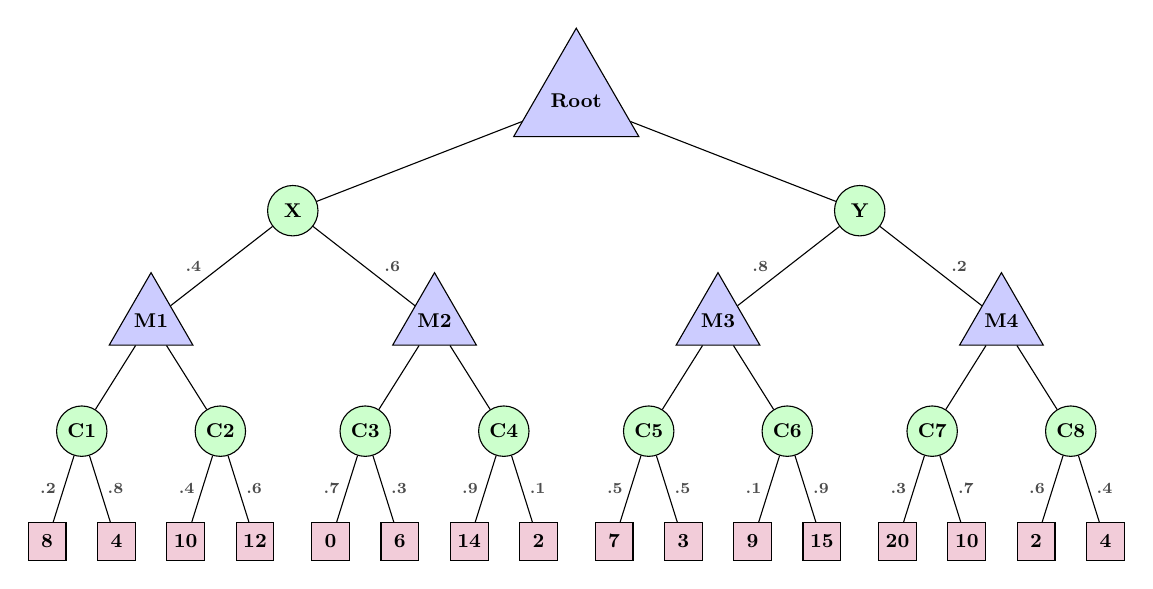
\begin{tikzpicture}[level distance=1.75cm,
  level 1/.style={sibling distance=9cm},
  level 2/.style={sibling distance=4.5cm},
  level 3/.style={sibling distance=2.2cm},
  level 4/.style={sibling distance=1.1cm},
  scale=0.8, every node/.style={transform shape}]
  
  \node[maxnode] {Root}
    child {node[chancenode] {X}
      child {node[maxnode] {M1}
        child {node[chancenode] {C1}
          child {node[terminal] {8} edge from parent node[left, prob] {.2}}
          child {node[terminal] {4} edge from parent node[right, prob] {.8}}
        }
        child {node[chancenode] {C2}
          child {node[terminal] {10} edge from parent node[left, prob] {.4}}
          child {node[terminal] {12} edge from parent node[right, prob] {.6}}
        }
        edge from parent node[left, prob, xshift=-0.2cm] {.4}
      }
      child {node[maxnode] {M2}
        child {node[chancenode] {C3}
          child {node[terminal] {0} edge from parent node[left, prob] {.7}}
          child {node[terminal] {6} edge from parent node[right, prob] {.3}}
        }
        child {node[chancenode] {C4}
          child {node[terminal] {14} edge from parent node[left, prob] {.9}}
          child {node[terminal] {2} edge from parent node[right, prob] {.1}}
        }
        edge from parent node[right, prob, xshift=0.2cm] {.6}
      }
    }
    child {node[chancenode] {Y}
      child {node[maxnode] {M3}
        child {node[chancenode] {C5}
          child {node[terminal] {7} edge from parent node[left, prob] {.5}}
          child {node[terminal] {3} edge from parent node[right, prob] {.5}}
        }
        child {node[chancenode] {C6}
          child {node[terminal] {9} edge from parent node[left, prob] {.1}}
          child {node[terminal] {15} edge from parent node[right, prob] {.9}}
        }
        edge from parent node[left, prob, xshift=-0.2cm] {.8}
      }
      child {node[maxnode] {M4}
        child {node[chancenode] {C7}
          child {node[terminal] {20} edge from parent node[left, prob] {.3}}
          child {node[terminal] {10} edge from parent node[right, prob] {.7}}
        }
        child {node[chancenode] {C8}
          child {node[terminal] {2} edge from parent node[left, prob] {.6}}
          child {node[terminal] {4} edge from parent node[right, prob] {.4}}
        }
        edge from parent node[right, prob, xshift=0.2cm] {.2}
      }
    };
\end{tikzpicture}
\end{center}

\begin{enumerate}[resume]
    \item \textbf{Layer 4 Expected Values:} Calculate the expected utility for chance nodes C1 through C8.
    \vspace{4cm}

    \item \textbf{Layer 3 Max Values:} What values will Max nodes M1, M2, M3, and M4 choose?
    \vspace{2cm}

    \item \textbf{Layer 2 Expected Values:} Calculate the expected utility for chance nodes X and Y.
    \vspace{2.5cm}

    \item \textbf{Root Node (Max):} What is the final expectimax value at the Root, and which path (towards X or Y) is optimal?
    \vspace{2cm}
\end{enumerate}
\end{document}